\chapter{协议实现}

以下将分别介绍本次实验的五个部分的具体实现方式。

\section{第一周——实现简单的 echo web server}

第一周的协议实现主要分为“消息解析”和“消息反馈” 两个部分。

\subsection{消息解析}

\begin{figure}[htbp!]
    \centering
    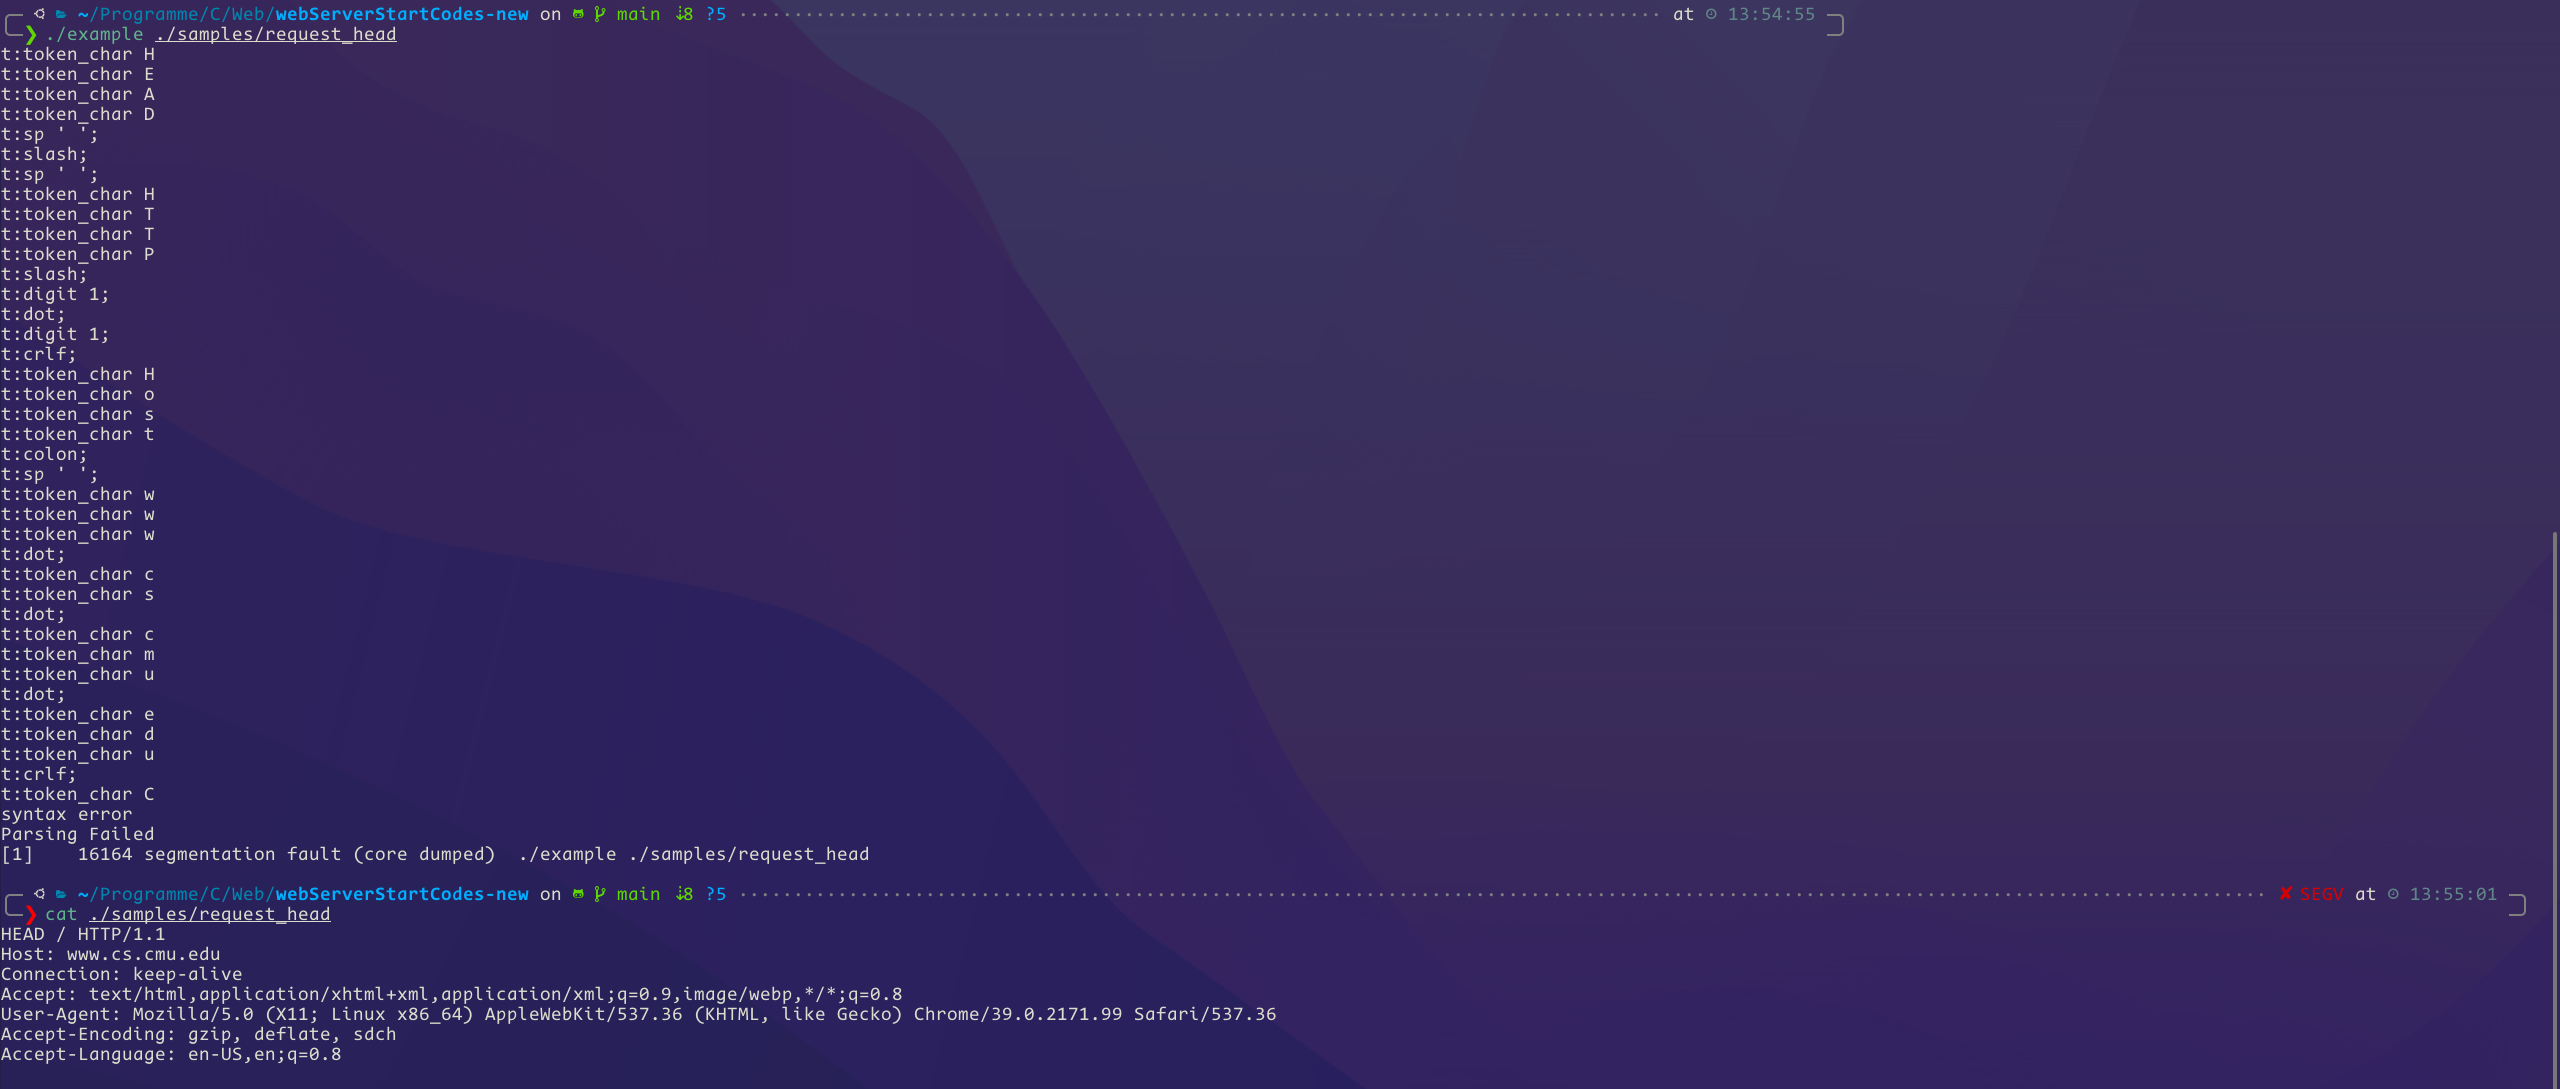
\includegraphics[width=4.5in]{segmentFault.png}
    \caption{Segment Fault}\label{fig:segmentfault}
    \vspace{-1em}
\end{figure}

如图\ref{fig:segmentfault},通过 example.c 的测试,我们发现了第一个错误: Segment fault,且该错误总是在解析第三行消息时出现。

通过对 parser.y 和 parse.h 文件的理解,我们认为此问题应该出自其 Request 中 Request\_header,它在最初定义时是一个指针 *header,所以在解析第二行时没有错误,而在进行第三行即以后的解释时,如果不进行人为的空间分配,则当然会出现上述的 Segment Fault。

所以对于这个问题,我们只需在 parser.y 中进行修改,增加 realloc 的函数,对 header 进行扩容,并且相应的 grammar 与之对应即可。

当然,还可以在 example.c 中处理一下返回错误的情况,避免直接访问 NULL 的空间导致 Segment Fault。使用批量脚本测试则效果如图\ref{fig:maketestexample}。

\begin{figure}[htbp!]
    \centering
    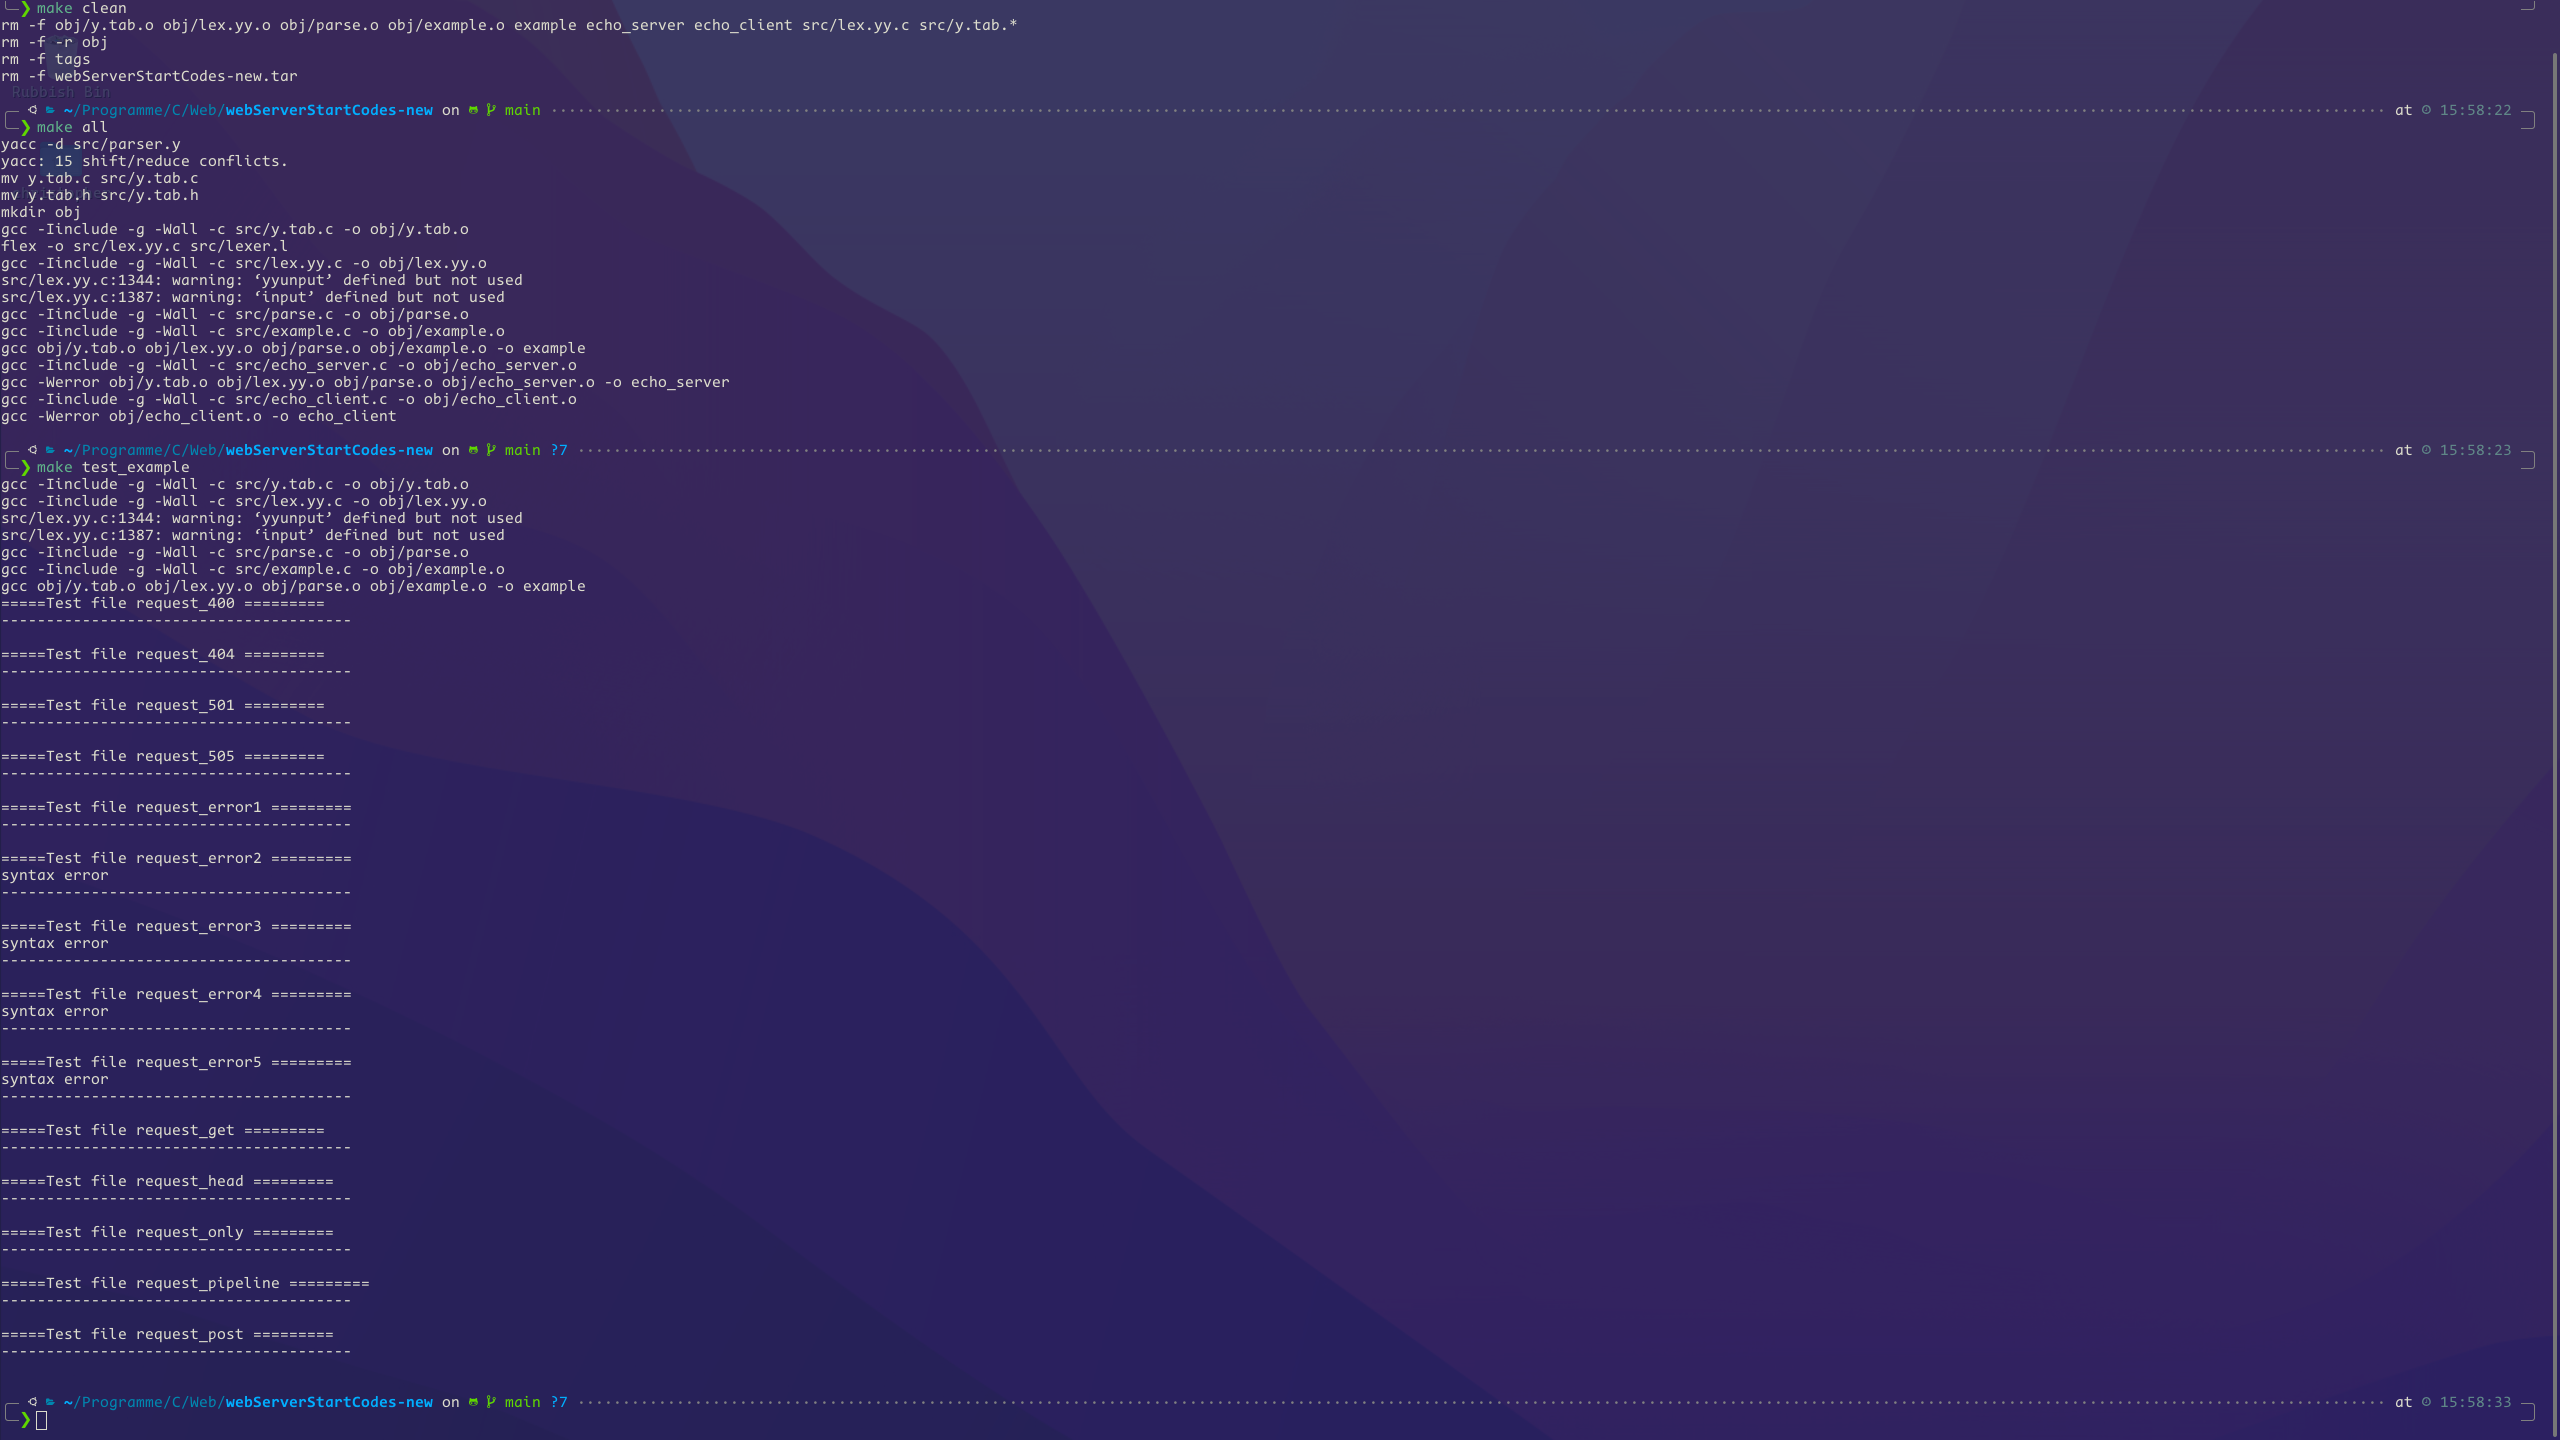
\includegraphics[width=4.5in]{make_test_example.png}
    \caption{Example Test}\label{fig:maketestexample}
    \vspace{-1em}
\end{figure}

\subsection{消息反馈}

在完成消息解析后,我们对 echo\_server.c 进行编程,完成消息的解析、处理与返回。研读源代码,梳理出如 "echo\_server" 代码段的伪代码。

我们只需要在第 7 行 "TODO: DEAL WITH MESSAGE" 处增加如代码段 “处理数据” 的 “解析、分类、封装返回值” 即可。

\begin{itemize}
    \item 具体而言,先通过 example.c 一样的方法解析 buf 中收到的数据。在该步骤中,可能会出现依赖问题,对此我们需要在 Makefile 中增加相关的依赖。让 echo\_server 在连接时加上 parse.o 的文件即可。
    \item 得到 request 后,我们对 request 的两种情况进行分析
    \item 如果 request 为 NULL,则解析不成功,即返回 400 错误
    \item 如果 reqeust 成功,但是发现其中 method 暂不支持,则返回 500 错误
    \item 否则直接返回受到的数据
\end{itemize}

\begin{lstlisting}[language=python, name={echo_server}]
create socket
bind socket
listen on socket
while(1):
    accept connection
    while(recieve message):
        TODO: DEAL WITH MESSAGE
        send back
    close client socket
close socket
\end{lstlisting}
    
\begin{lstlisting}[language=python, name={dealing with Data}]
def deal_with_request(buf):
    Request *request = parse(buf, BUF_SIZE, 8192)
    if request is NULL:
        return _400msg
    if method_not_support:
        return _500msg
    return buf
\end{lstlisting}

\section{第二周——实现 HEAD、GET、POST 方法}
第二周的协议实现主要分为“基本方法实现”、“缓冲区处理”、“日志记录模块”、“读写文件”这四个部分。

\subsection{方法实现}

服务器处理请求的方法被集中封装到文件 response.c 和 response.h 中。函数原型如图\ref{fig:Responsech} 所示。

具体而言,liso\_server 首先使用 while 来接收信息,存储到 buffer 中(此处采用自定义的动态缓存,在下一节详细介绍)。然后通过一个 strstr() 函数获取确定一个完整的请求后,将它加载到动态缓存 dbuf 中,并调用函数 handle\_request 处理,返回的信息将继续通过 dbuf 带出。由于测试集的要求,此处不需要实现 Persistent Connection 中对连接情况的判断。下面将分别介绍错误码和基本方法的实现。

\subsubsection{错误码}

\paragraph*{400}
400 错误是解析错误,由于之前在 Lab 1 已经实现了较为完备的 parse() 函数,于是在 Lab 2 中将不再 parse() 函数之内做修改。\textbf{首先},通过图\ref{fig:Responsech}左侧 第 37 行调用 parse() 函数对请求进行解析,并通过第 40 行的判断确定一个 400 的错误,并随即调用函数 handle\_400 处理之。\textbf{然后},通过对自定义函数的调用,对动态缓冲数组 dbuf 进行清空、加载返回信息等操作。

\paragraph*{404}
404 错误是指无法找到请求的文件,目前只会在 HEAD 和 GET 方法处理时出现。在处理 GET 和 HEAD 请求时,我们会通过 stat 等函数对要请求的文件进行预处理,此时即可判断该文件是否存在、是否可读等权限问题,然后决定是否返回 404 错误。

\paragraph*{505}
505 错误是指协议版本不支持,通过图\ref{fig:Responsech} 左侧第 53 行判断 my\_http\_version 与请求的 version 是否相同即可。

\paragraph*{501}

501 错误是指请求方法不支持,也可以通过一个 switch 判断出来。此处的 method\_switch() 函数,将一个表示方法的字符串 ("GET", "POST", etc) 转化为图\ref{fig:Responsech} 右侧第 35 行定义的枚举类 METHOD。


\subsubsection{基本方法}

\paragraph*{HEAD} HEAD 方法的具体实现由函数 handle\_head() 实现。\textbf{首先},通过函数 strcmp() 判断请求路径是否为默认路径,如果是,则直接请求文件 index.html, 否则请求路径添加到子文件夹 "./static\_site" 之下。\textbf{然后},通过函数 stat() 判断是否为 404 错误。如果一切顺利,则通过在下一节介绍的动态缓冲区处理函数按照前文提到的格式,向返回值 dbuf 中添加一系列 response 和 headers。具体如图\ref{fig:handleHead} 所示。


\begin{figure}[htbp!]
    \centering
    \subfigure[Response.c 和 Response.h]{\label{fig:Responsech}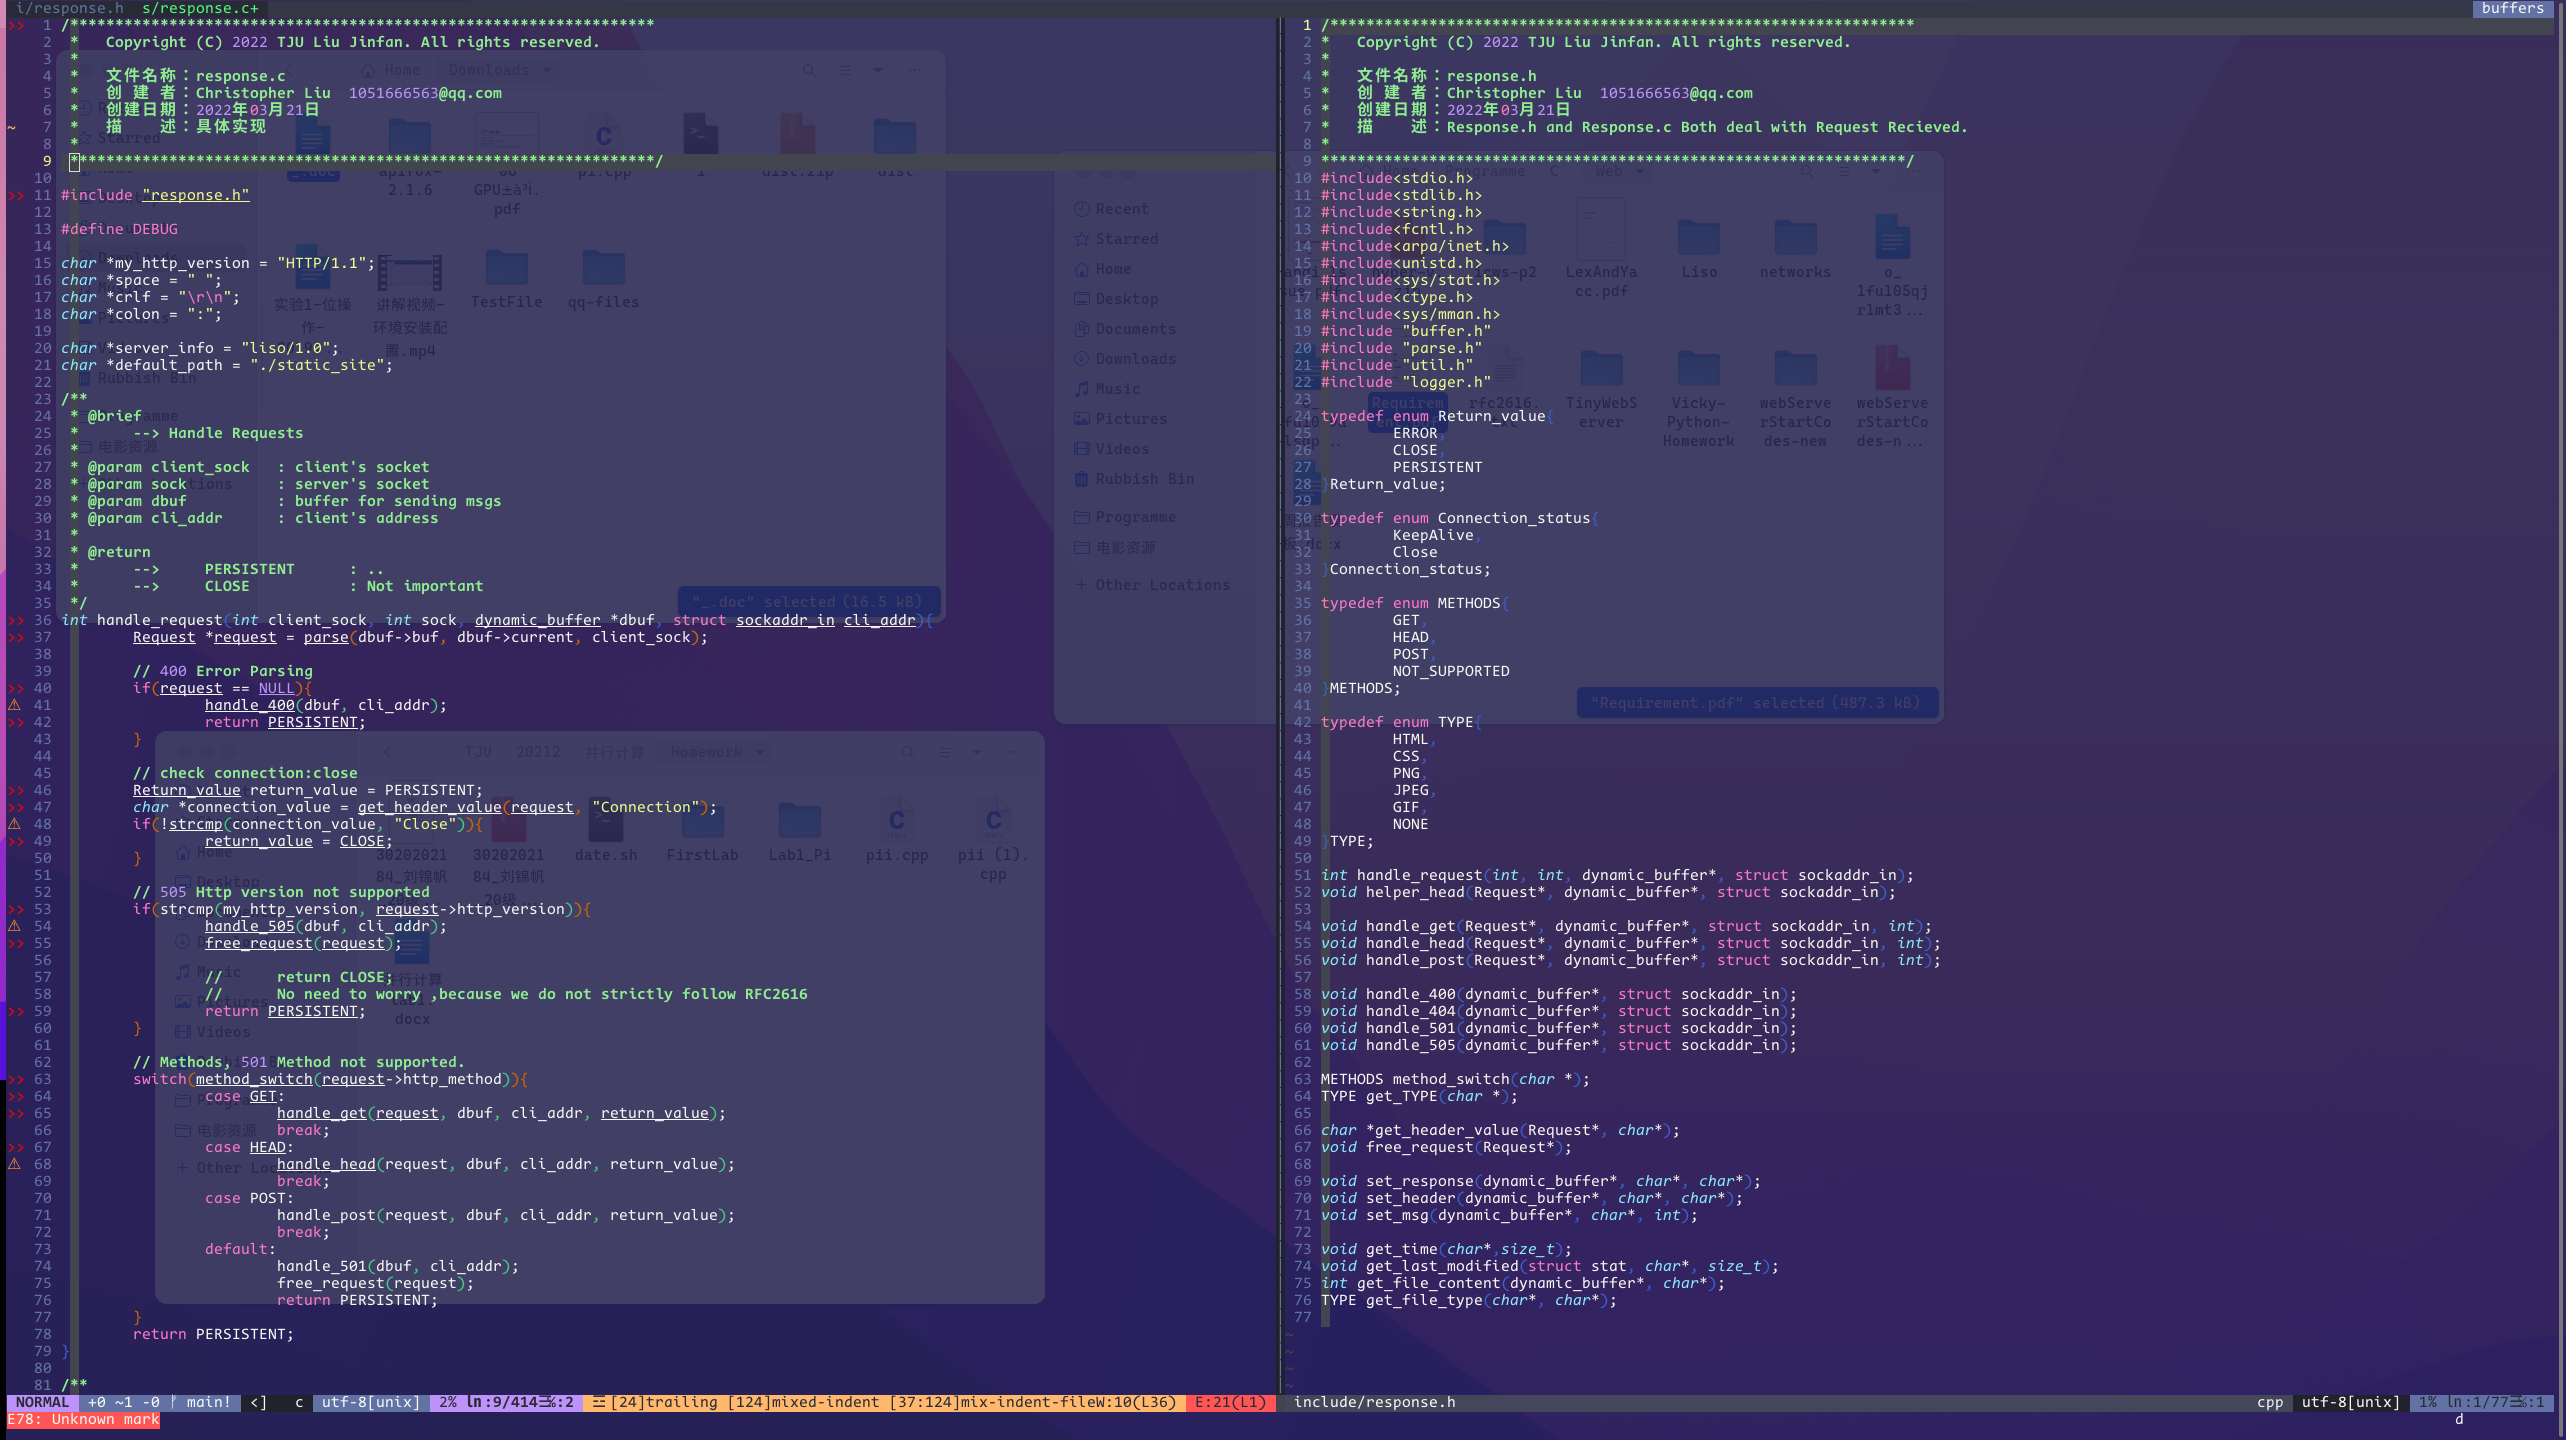
\includegraphics[width=5in]{responsech.png}}
    \subfigure[liso\_server.c 和 liso\_client.c]{\label{fig:liso}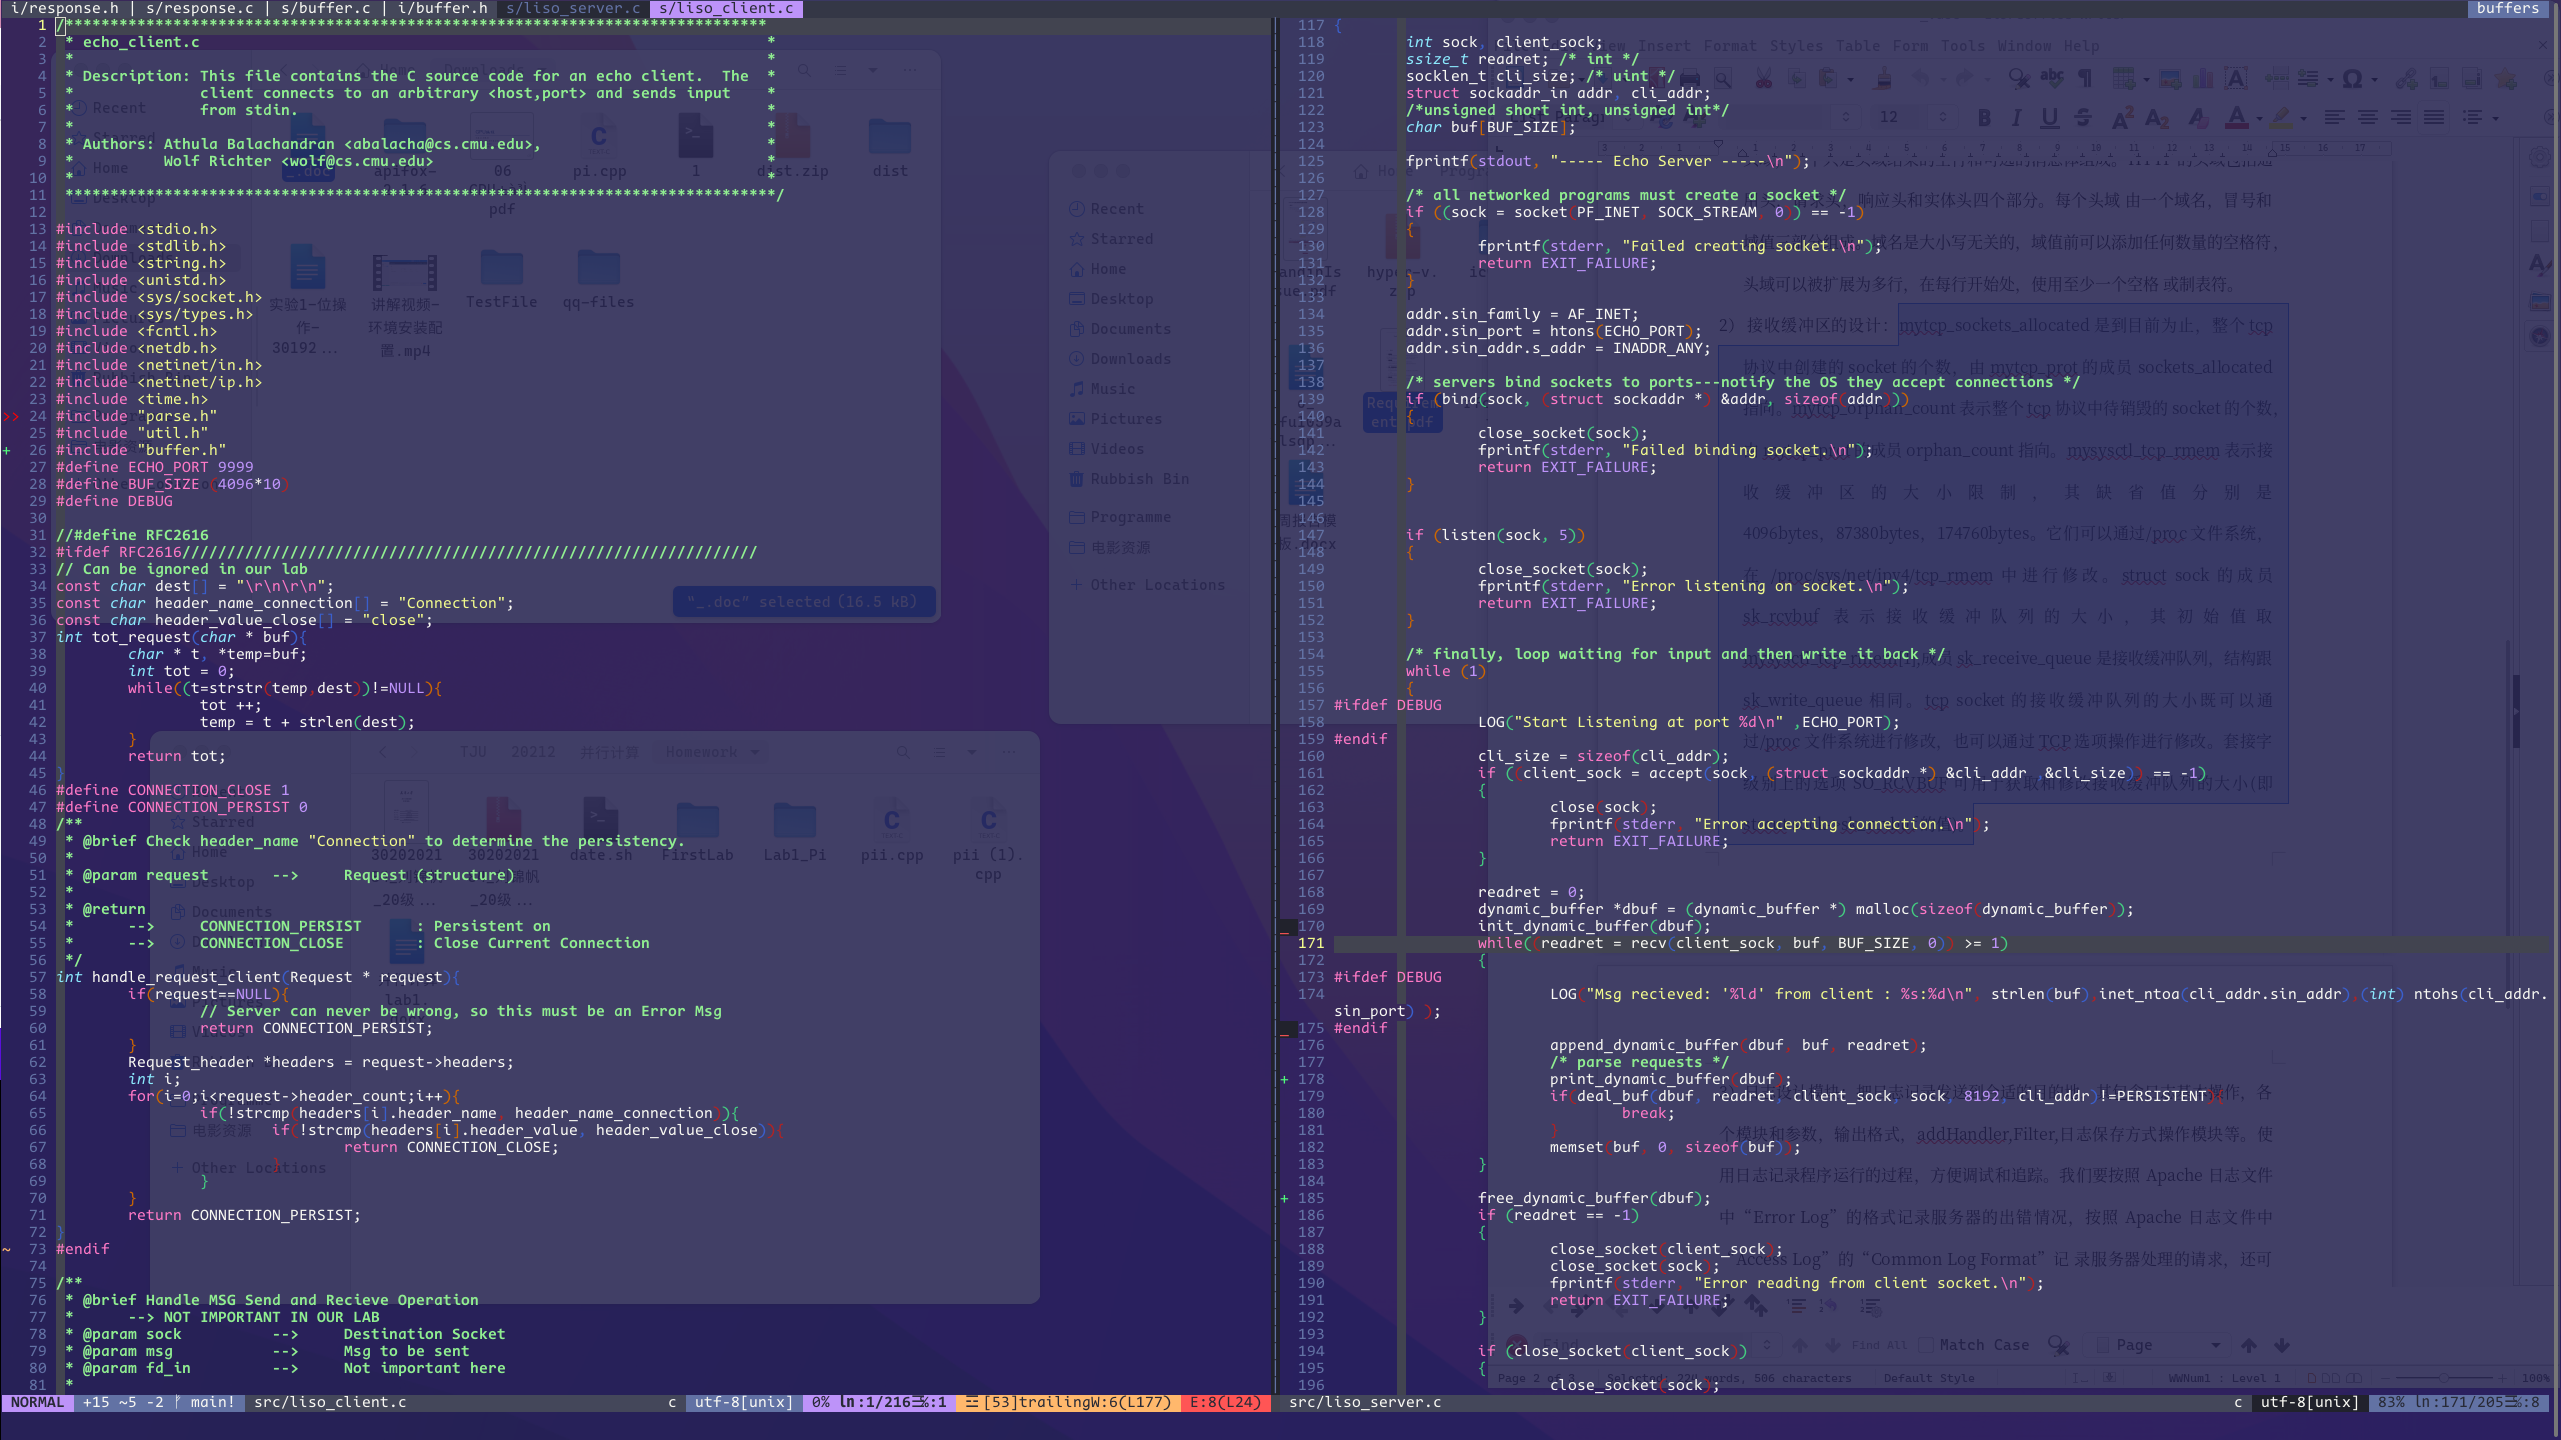
\includegraphics[width=5in]{liso.png}}
    \caption{核心代码}\label{fig:Main}
\end{figure}

\paragraph*{GET} GET 方法在 HEAD 方法的基础之上,添加了读取文件的操作,根据模块化变成的思想,我们将其封装到函数 get\_file\_content() 之中。为了实现对缓冲区的管理、避免 Segment Fault,我们仍先通过 stat 函数对文件情况做初步确定,并先对动态数组进行扩容,再读入文件。文件读入部分将在后续小节进行介绍。

\paragraph*{POST} POST 方法的实现,根据实验要求,直接返回接收到的报文,于是在判断没有 400,505,以及 501 错误之后,我们即可将携带请求信息的动态数组 dbuf 原路返回。

\subsection{妥善管理缓冲区}

由于 socket 编程本身的性质,在 send 函数中会主动的将信息拆分成合适大小再分别发送。所以我们只需要针对 \textbf{1.} 发送前,用户的缓冲区; \textbf{2.} 接收后集中存放的用户缓冲区; 两个缓冲区进行管理。

\subsubsection{动态数组定义与实现}
我们的策略,是通过自定义的动态数组实现对一个动态长度的缓冲区的支持。具体定义及部分实现如图\ref{fig:dynamicBuffer}所示。


部分结构体、函数介绍如下:

\paragraph*{struct dynamic\_buffer} 该结构体定义了一个基地址 *buf, 以及它的总大小 capacity 和当前大小 current。

\paragraph*{init\_dynamic\_buffer()} 该函数使用系统调用 malloc 将为一个新定义的动态数组分配由宏 "DEFAULT\_CAPACITY" 定义的空间。即对动态数组进行初始化。

\paragraph*{append\_dynamic\_buffer()} 该函数将一个字符串拼接到动态数组后面。首先判断当前空间是否够用,如果不够,则调用函数 realloc 为其增添空间,然后通过 memcpy() 函数,将新添加的字符串拼接到动态数组后面。


\subsubsection{动态数组使用}

动态数组的作用是解决缓冲区溢出问题,前文提到的两个可能出现溢出的地点,分别是读入文件时由于文件过大(或将其加入返回信息时)而溢出,另一个是在接收端虽然一次性接收的最大值由 BUF\_SIZE 控制,但是用户发送的请求大小不可定(例如 Lab3 中的 pipeline),导致缓冲区溢出。最终为了整体的和谐性,我们在大多数使用字符串数组的地方,都改用我们的动态数组。例如:

\paragraph*{读入文件时} 首先使用 stat() 获取文件大小,然后调用函数 add\_dynamic\_buffer() 函数对我们的动态数组进行可用空间的检验。最后再通过 read() 或者 mmap() 将文件写入动态数组。

\paragraph*{Server 端} 在 server 端,我们使用动态数组,存储即将返回给 client 的信息。由于 GET 可能会请求大小超标的文件,于是我们通过有保护机制的动态数组,安全地对它进行读取与返回。

\paragraph*{接收 socket 信息时} 由前文提到地 recv() 函数的性质,我们知道应该通过 while 来不断读取管道里的信息,如图\ref{fig:liso} 右侧第 171 行。通过 append\_dynamic\_buffer() 函数,将读取的信息添加到当前动态数组 dbuf 中。每次处理缓冲区,即是对 dbuf 中的数据进行拆分(确定一份请求报文)、解析与返回,最后调用 update\_dynamic\_buffer() 函数,将该报文从动态数组中丢弃。最大限度地节约空间,并解决缓冲区溢出问题。
\begin{figure}[htbp!]
    \centering
    \subfigure[dynamic\_buffer.c 和 dynamic\_buffer.h]{\label{fig:dynamicBuffer}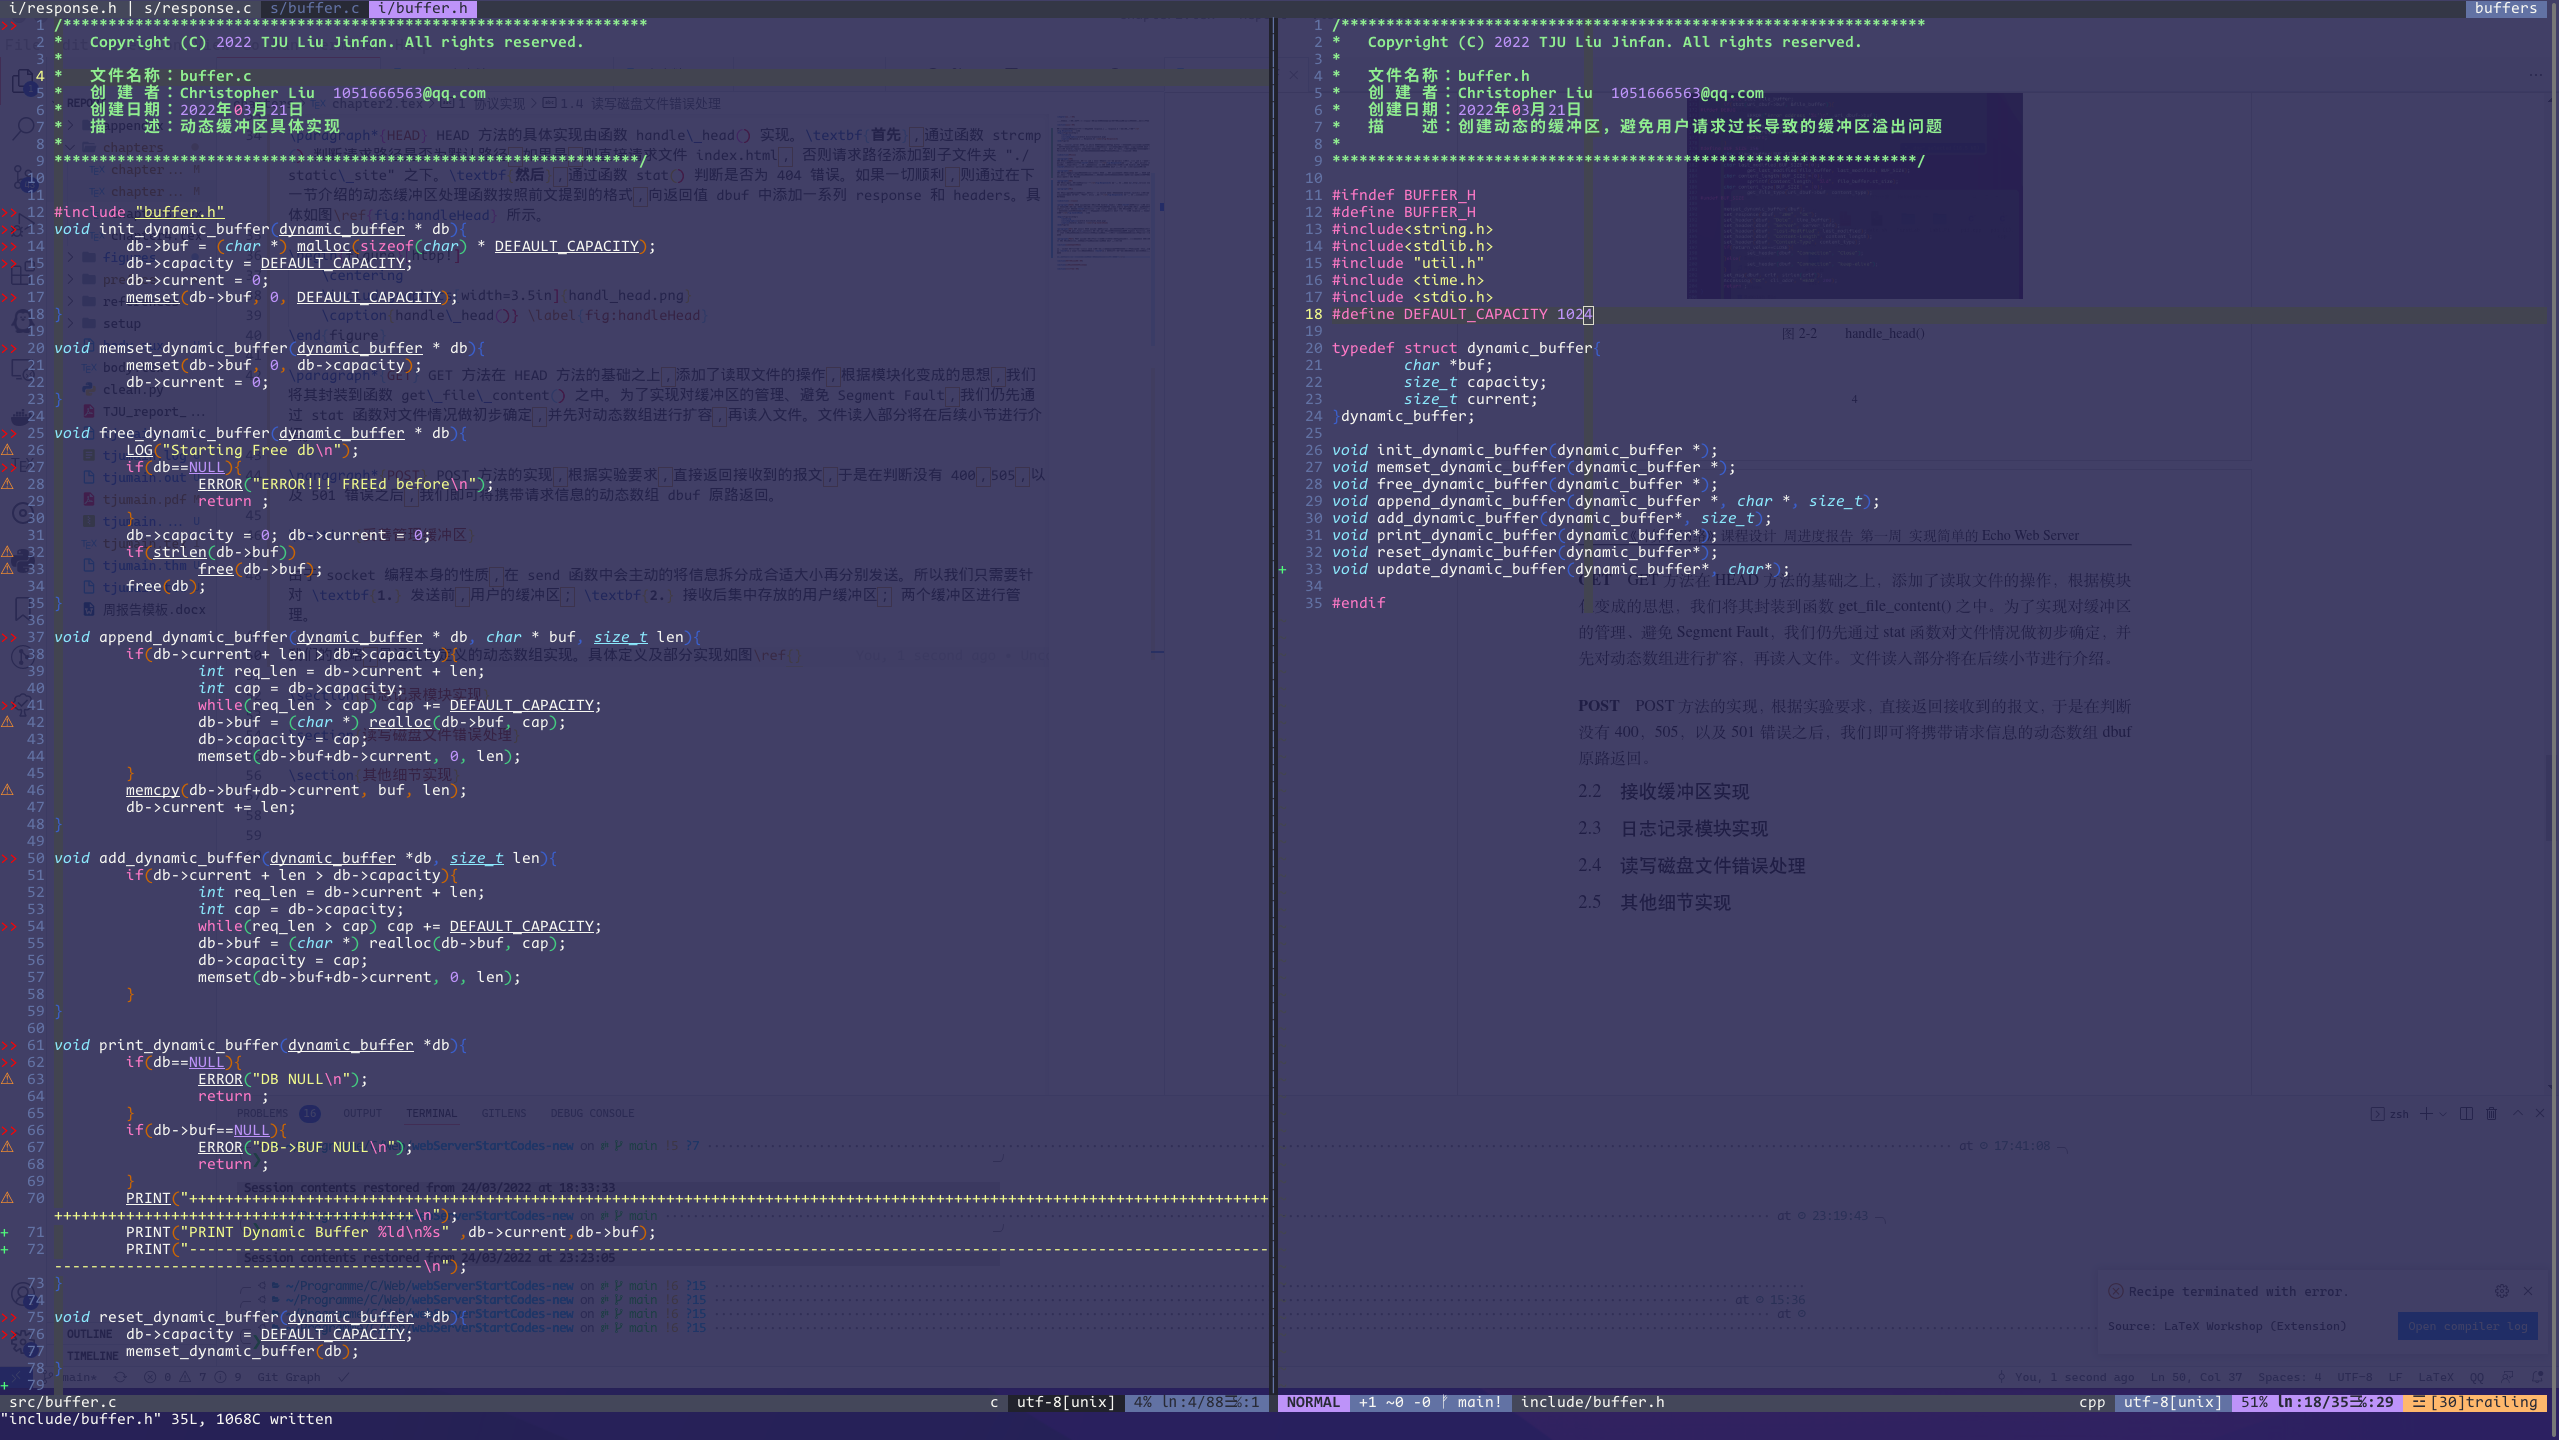
\includegraphics[width=5.5in]{dynamic_buffer.png}}
    \subfigure[handle\_head 函数]{\label{fig:handleHead}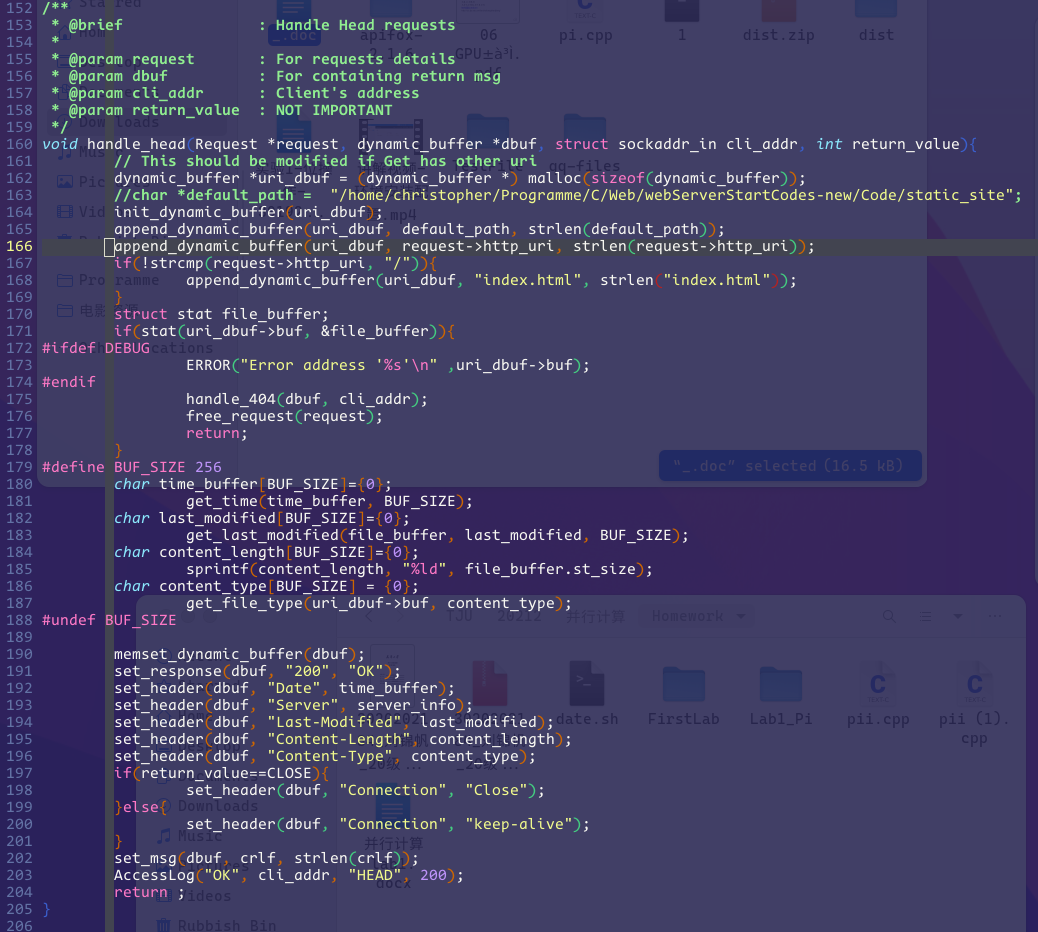
\includegraphics[width=2.1in]{handl_head.png}}
    \subfigure[日志文件]{\label{fig:log}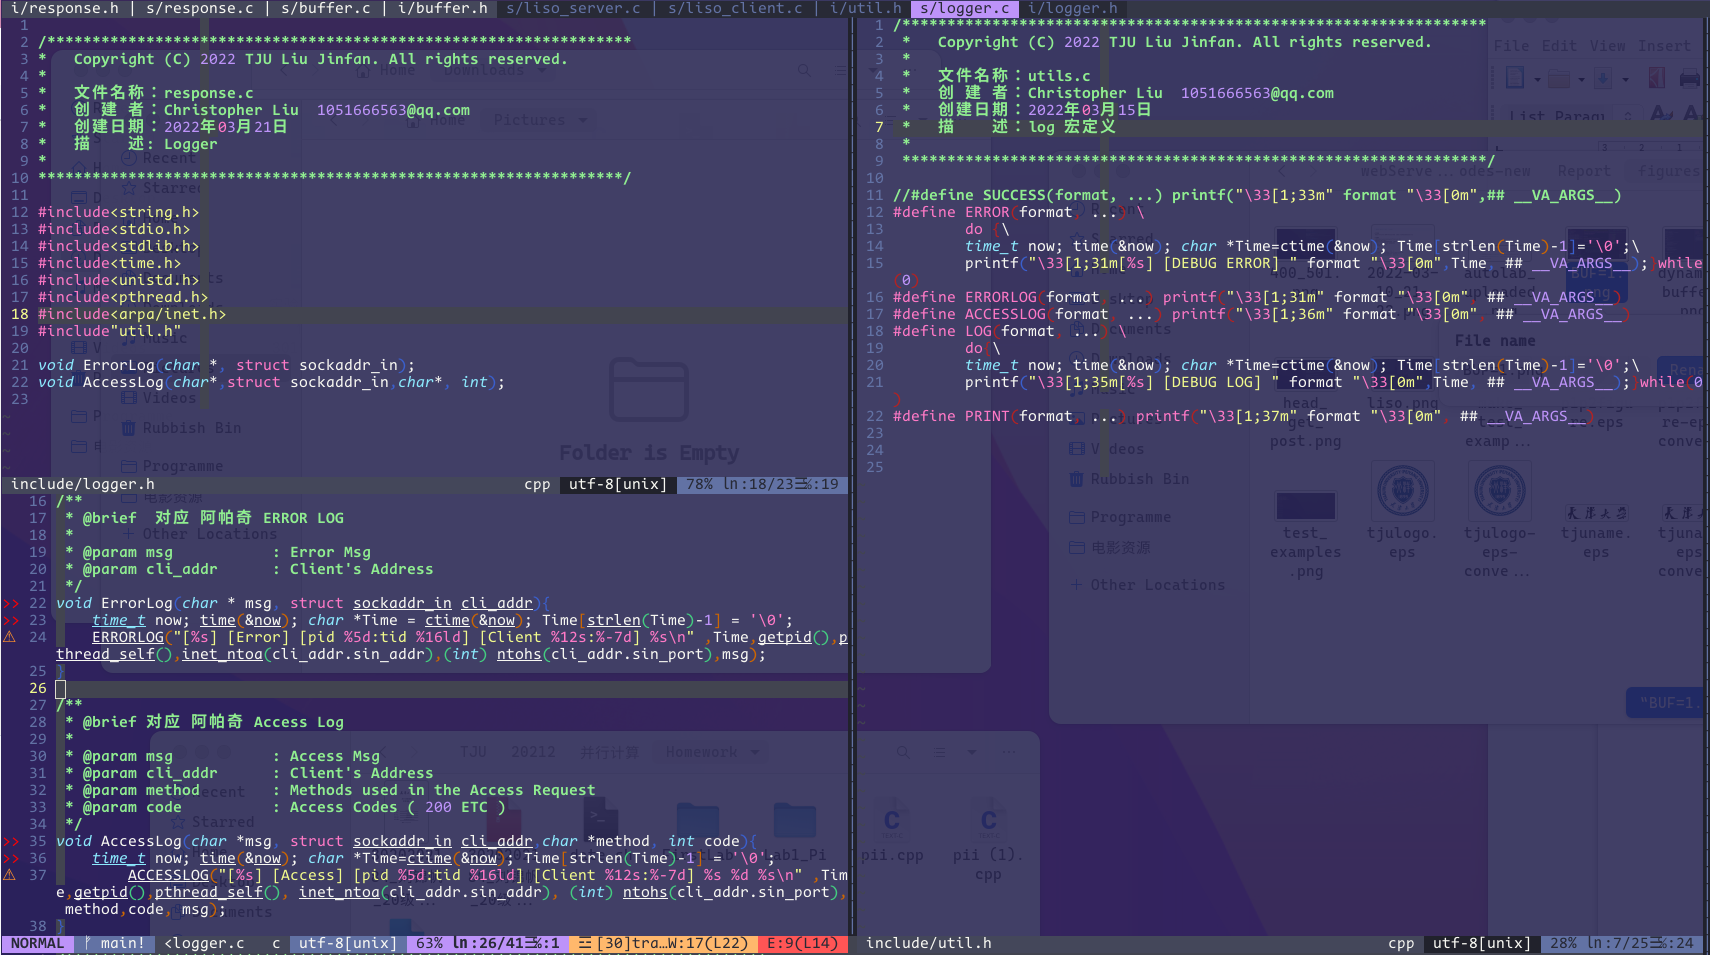
\includegraphics[width=3.3in]{log.png}}
    \caption{动态数组、日志文件以及 Handle Head 函数}\label{fig:Chapter2}
\end{figure}


\subsubsection*{验证}
如图\ref{fig:buffer},即使将缓冲区大小设置为 1,我们的 server 依旧正常处理并返回信息(测试样例为 pipeline,由于和 Persistent Connection 相关联,故一起实现了)。
\begin{figure}[htbp!]
    \centering
    \subfigure[buffer\_test,BUF\_SIZE=1]{\label{fig:buffer}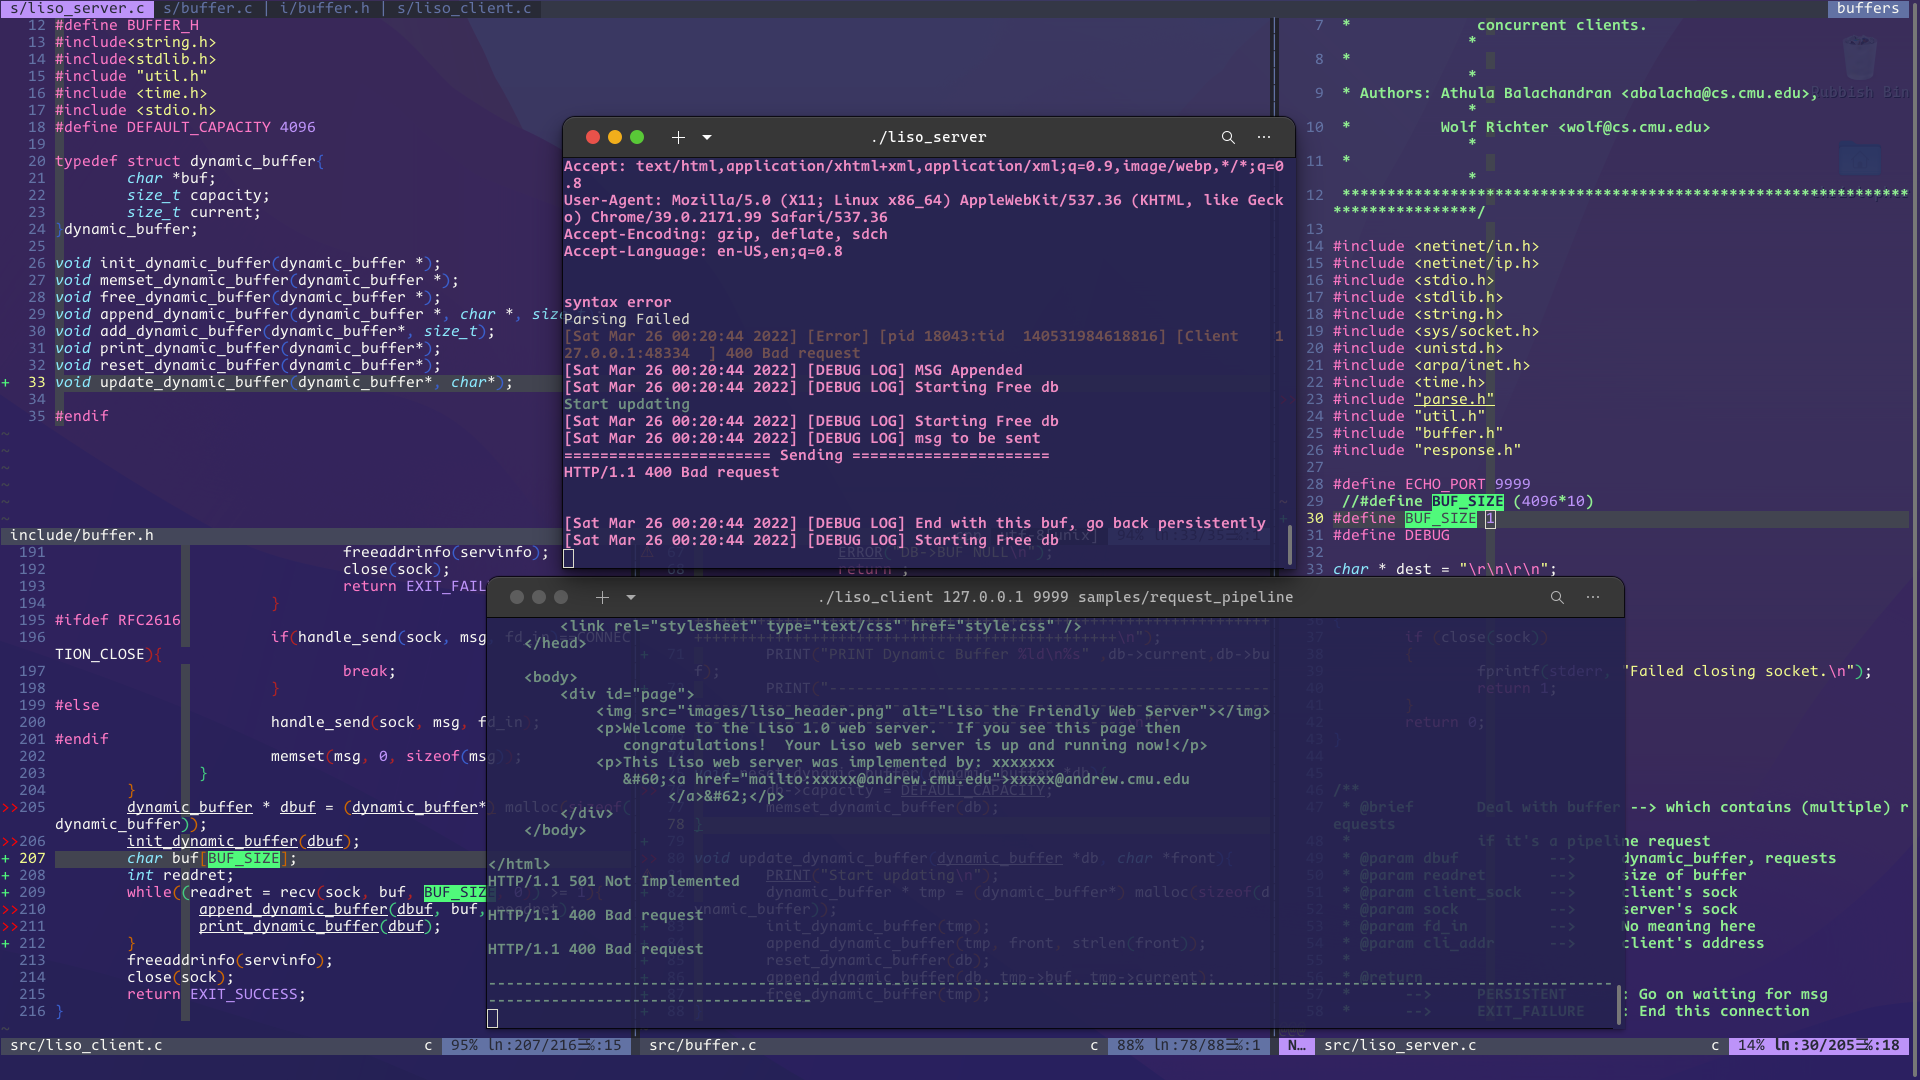
\includegraphics[width=3.5in]{BUF=1.png}}
    \subfigure[get\_file\_content函数]{\label{fig:openfile}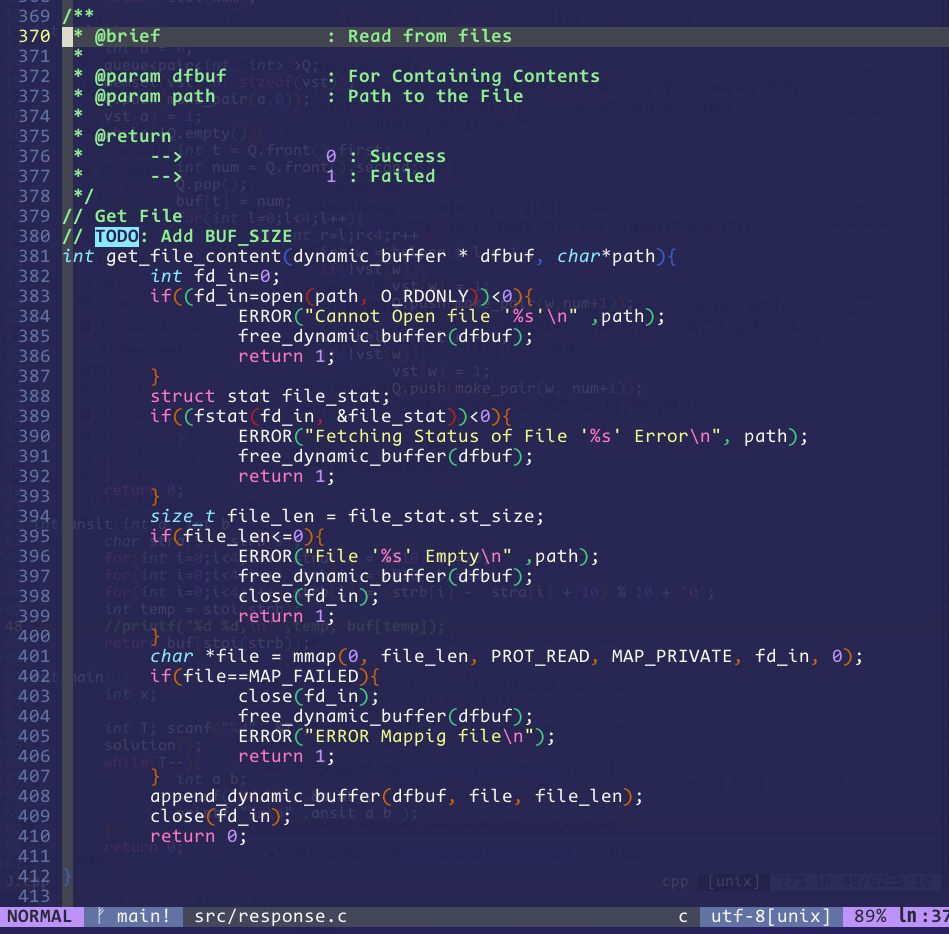
\includegraphics[width=2in]{getFileContent.png}}
    \caption{测试 buffer 以及 get\_file\_content 函数}\label{fig:Chapter2.2}
\end{figure}

\subsection{日志记录模块实现}
日志记录模块借用了 Apache 标准,使用 C 宏定义完成第一层封装,采用 logger.c 与 logger.h 配合,进行向特定文件的输入,实现了 log 的可跟踪性。具体宏定义如图\ref{fig:log} 所示。

\subsection{读写磁盘文件错误处理}
只有 GET 和 HEAD 请求涉及对文件的处理。根据之前的描述,我们首先使用 stat() 函数对磁盘文件进行试探性的访问。如果在此时出错,可能有 1. 路径不存在; 2. 没有查看权限。在服务器看来,我们只需返回 404 错误即可。

在 GET 的处理中,我们还需对文件进行读取,此时可能又会产生 3. 无法打开的错误; 4. 文件为空;以及 5. 无法正确映射到内存;等问题(由于我们使用了上一节提到的动态数组,不会存在溢出问题)。

考虑完上述问题,我们实现了如图\ref{fig:openfile} 的代码。

\section{第三周——实现HTTP的并发请求}

第三周的实现较为简单。由于在 Lab2 中我们实现了缓冲区的自动化更新、防溢出。可以支持任意大小的文件传入。所以本周的任务中,我们只需要关注如何将收到的信息拆分为单个单个的报文。然后处理之即可。

我们的实现方式,是通过函数 strstr() 获得拆分每个报文。 strstr(str,dest) 函数得到 dest 在 str 第一次出现的地址。于是就能通过 strstr() 得到报文结束前 " \textbackslash r\textbackslash n\textbackslash r\textbackslash n "的位置。然后通过简单的字符串处理,就能开始处理单个报文了。部分代码如图\ref{fig:liso_server_pipelining}。

\begin{figure}[htbp!]
    \centering
    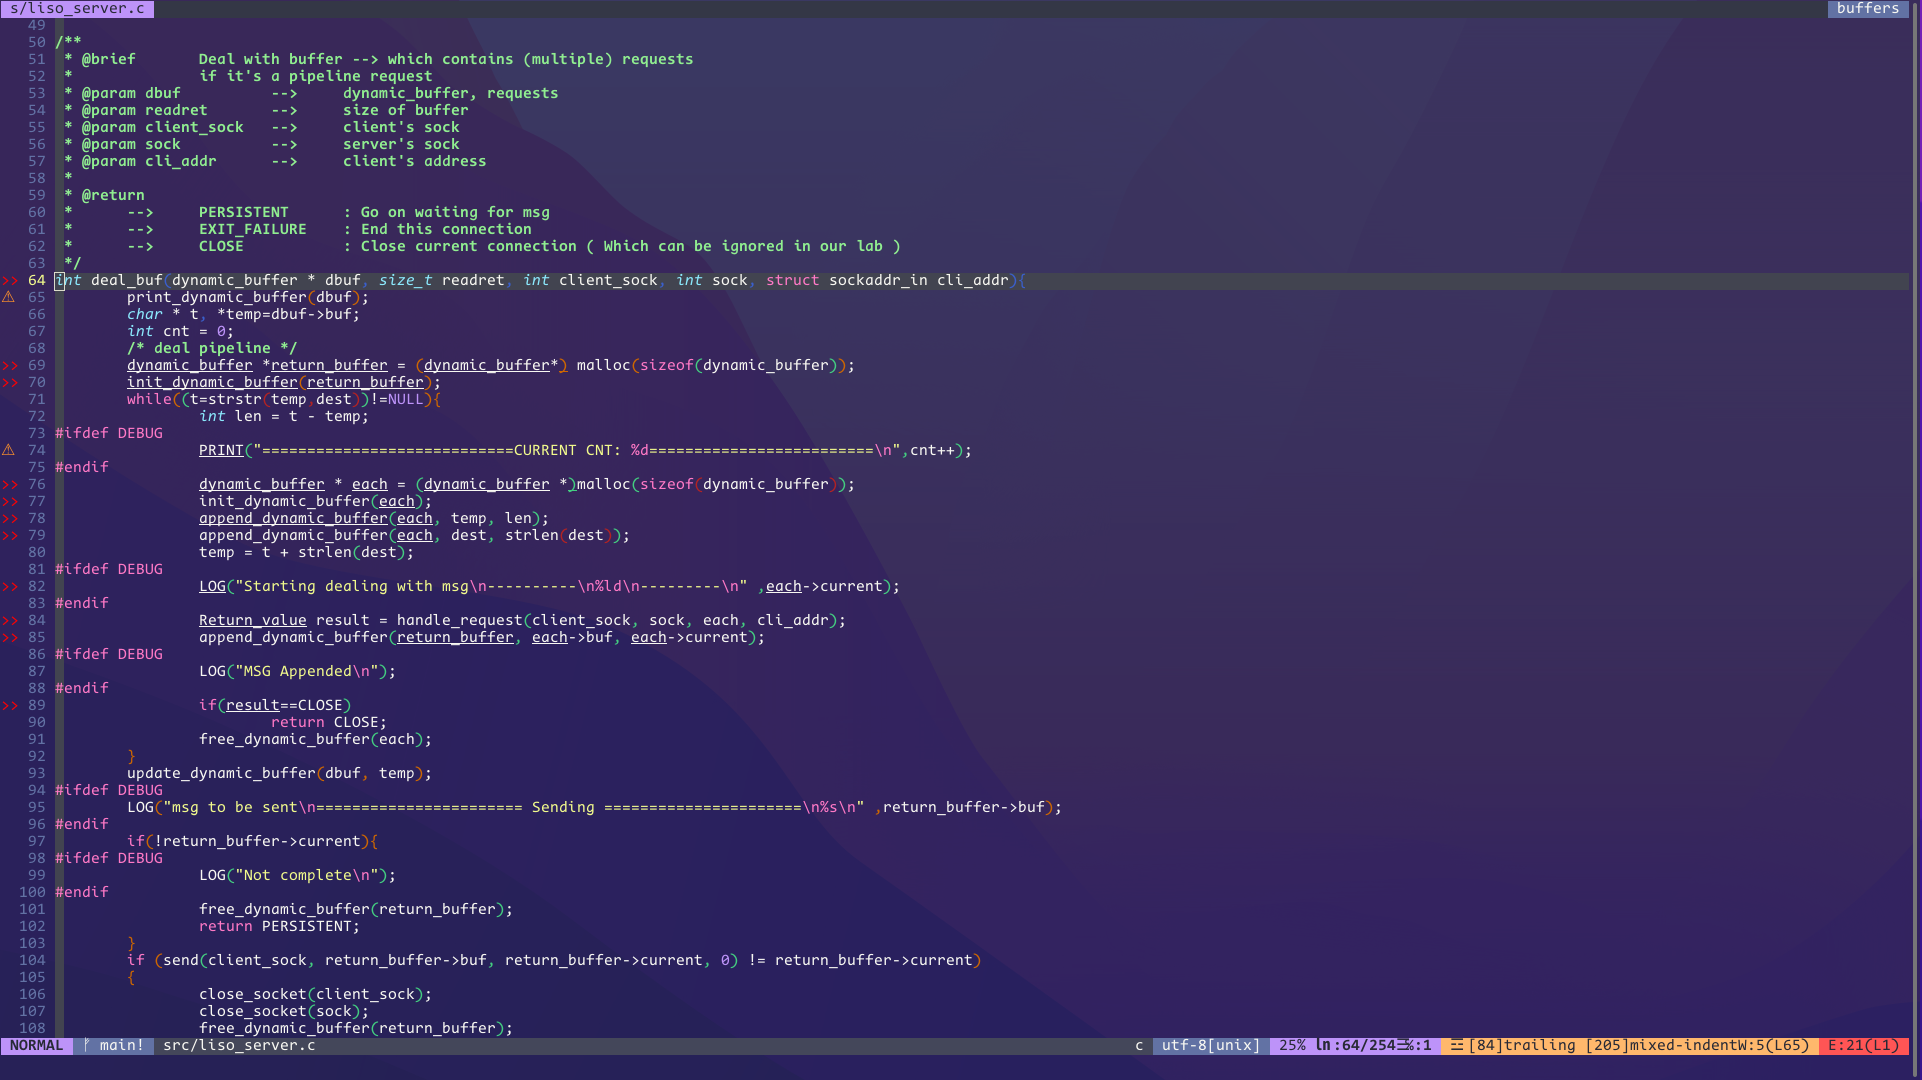
\includegraphics[width=5.6in]{liso_server_pipelining.png}
    \caption{Liso Server Pipelining}\label{fig:liso_server_pipelining}
\end{figure}

\section{第四周——实现多个客户端的并发处理}

第四周修改的主要是 liso\_server 的接收请求部分的代码。在 while(1) 的服务器处理循环中添加以 select 开头的预处理等操作,使服务器能够在等待一个客户端发送下一个请求时,同时处理来自其他客户端的请求,使服务器能够同时处理多个并发的客户端。

流程图如图\ref{fig:MultipleChart}所示。首先使用 cnt=select(MAX\_FD\_SIZE+1, \&tmp\_fds, NULL, NULL, NULL) 获取当前总共有多少个客户端有请求,同时将他们的文件描述符添加到类型为 fd\_set 的集合中,将用户总数返回给 cnt 变量。

然后循环遍历 fd\_set 集合中 0-MAX\_FD\_SIZE 个位置。通过函数 FD\_ISSET() 判断当前位是否有客户。如果有客户,则进行处理,否则跳过。

在处理时,先判断其文件描述符是否和服务器的 sock 相同,如果相同则表明是一个新的连接,需要进行 accept 操作,并为其分配一个新的文件描述符。如果和服务器的 sock 不相同,则按照一般流程处理。如果使用 select 选择了这个客户,且后续 recv 函数接收到的信息长度为 0,我们就可以认为这个客户已经离去,可以关掉它的 socket 了。

和前几次的一个小区别在于服务器需要为每个客户分配一个私有的空间来存储它的地址、端口以及缓存。对此,我们的实现方式,是使用地址类型和动态伸缩的数组。(也可以使用结构体,不过原理是一样的)。

\section{选做——CGI}

CGI 的实现将标志着我们的 Liso Server 走向成熟。能支持 CGI 程序的调用,标志着 Liso Server 拥有无穷的扩展性,不仅能够完成基本的报文解析、GET 消息的回传,还能支持多种应用。在我们的设计中,我们采用了前后端分离的思想,将 CGI 程序设计为后端应用,提供给在服务器端实现的 CGI 接口调用,为前端的请求服务。

具体而言,我们通过在第三部分介绍的数据结构 kv.[c|h] 来方便地对环境变量以及参数进行设置与传递。借鉴 cgi 文件夹中的例子,我们完成了全栈的开发。
\paragraph*{前端部分} 我们设计了 HTML 网页来与客户交互。通过修改 index.html 的代码,用“表单”将我们的 POST 和 GET 请求方法的页面入口放进去并实现跳转。在实际的测试页面,我们通过 JavaScript 的 "XMLHttpRequest()" 方法向我们的服务器发送 cgi 请求,并通过 document 方法对页面的信息进行动态的修改。

\paragraph*{接口部分} 后端设计的接口为两个,一个 "/cgi/register.py" 另一个为 "/cgi/login.py" 接口文档如图\ref{fig:CGIPORT} 所示。

\begin{figure}[htbp!]
    \centering
    \subfigure[CGI 登陆接口文档]{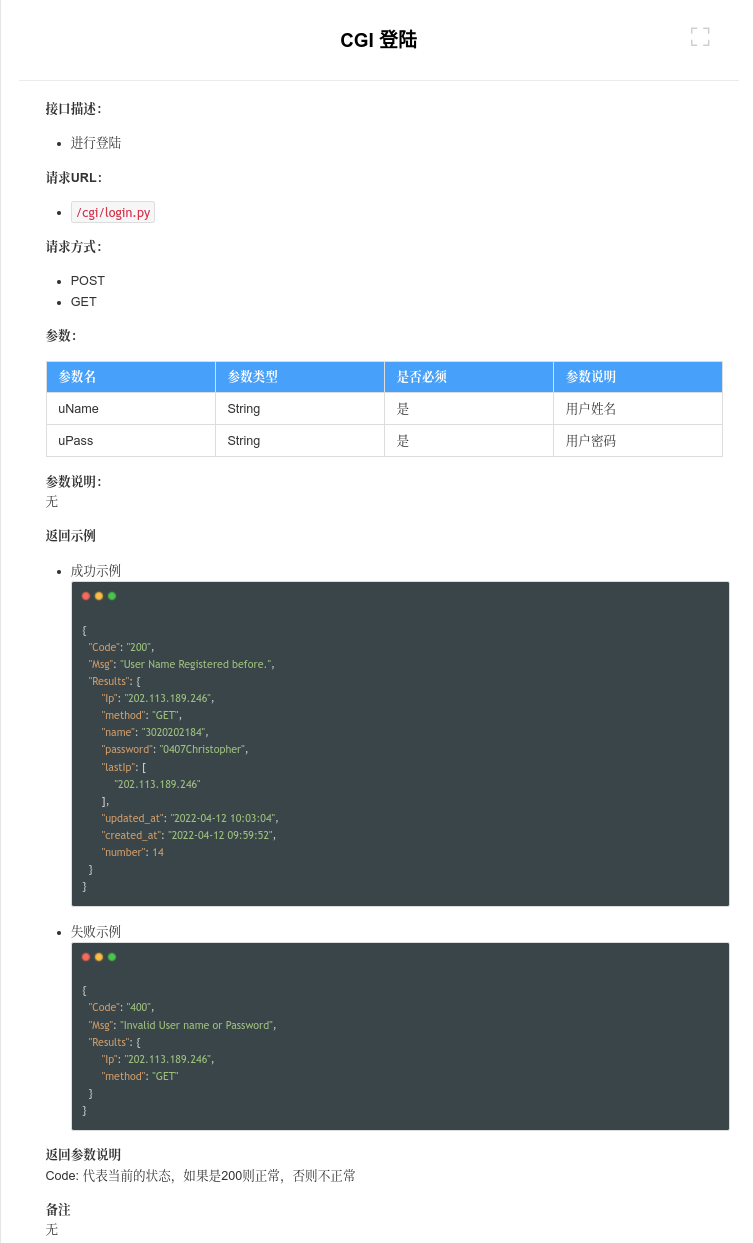
\includegraphics[width=2.5in]{CGILogin.png}\label{fig:cgiLogin}}
    \subfigure[CGI 注册文档]{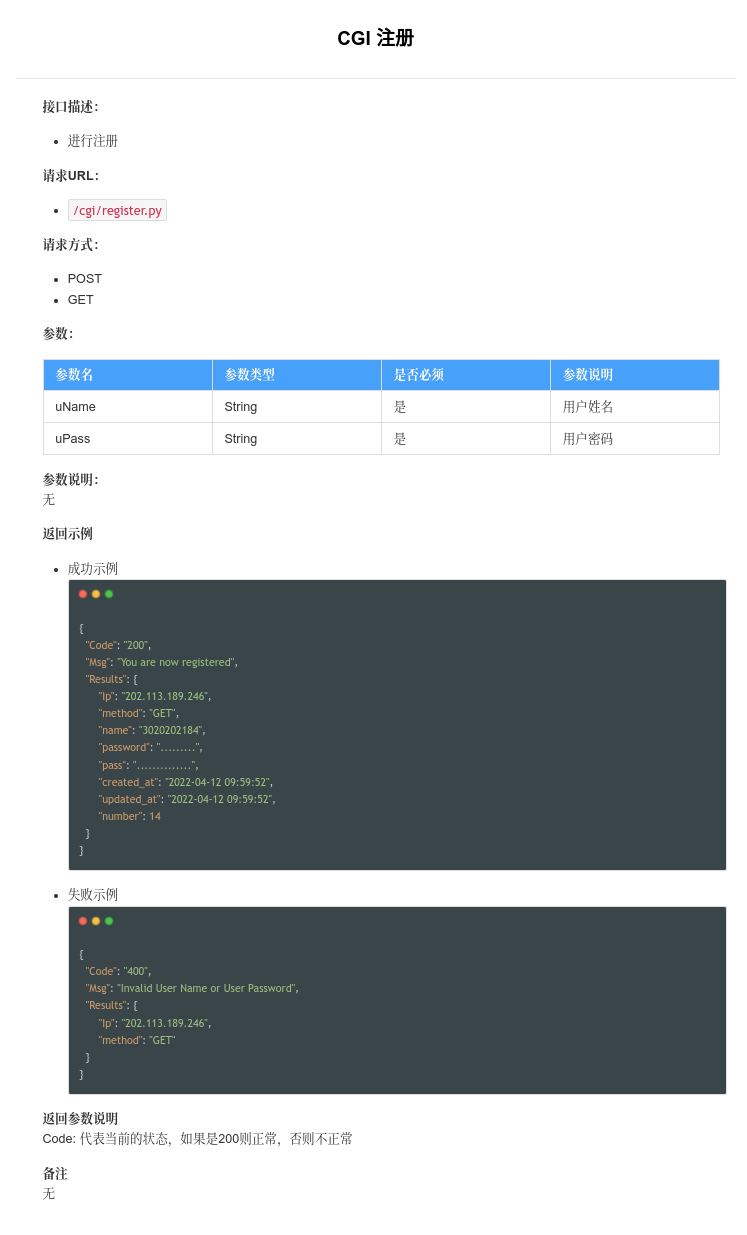
\includegraphics[width=2.5in]{CGIRegister.png}\label{fig:cgiRegister}}
    \caption{CGI 程序接口文档} \label{fig:CGIPORT}
\end{figure}


\paragraph*{后端部分} 设计了后端数据库结构(如图\ref{fig:database} 所示)来存储用户信息,实现了两个 Python 程序,分别处理用户注册和登陆的事务。Python 程序中没有采用高级的编程架构,只采用了基本的编程逻辑:使用 pymysql 库对数据库进行连接,然后通过相应的接口对数据库进行操作。进行数据库操作前需要检查参数是不是空的,避免数据库错误。同时还需要检查有没有数据库注入攻击的情况。对于返回类,我们通过一个“字典”类型的数据结构封装需要传回的信息。对于前端来说,受到的信息就是 Json 格式,能够很方便地通过相关方法进行参数的调用和访问。

\begin{figure}[htbp!]
    \centering
    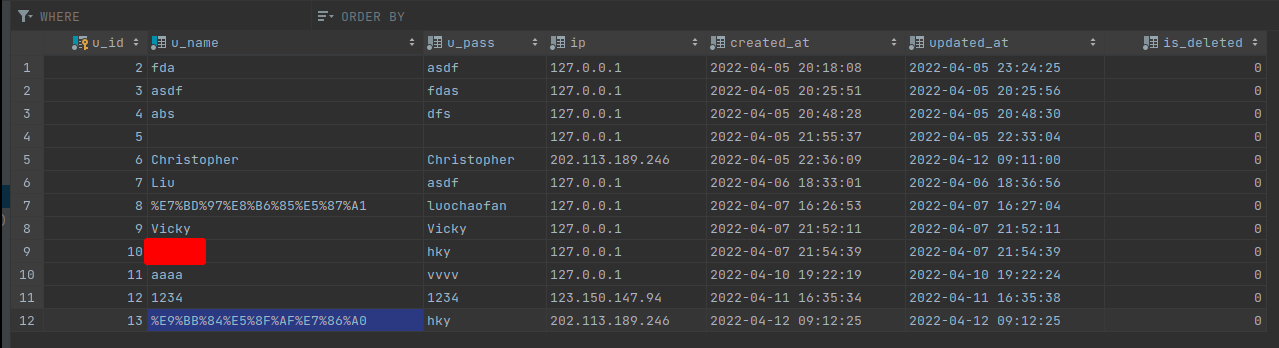
\includegraphics[width=5.6in]{database.png}
    \caption{Database for CGI}\label{fig:database}
\end{figure}
